\chapter{Introdução}

Ao longo dos anos, os astrônomos achavam que o nosso planeta, as estrelas e alguns intrigantes corpos celestes observados no céu, chamados de ``nebulosas'', constituíam nossa Via Láctea (expressão do grego helenístico \emph{galaxias kuklos}, em português ciclo leitoso) e eram o universo como um todo. No século XVIII, o filósofo alemão Immanuel Kant em sua obra História Natural Universal e Teoria dos Céus \cite{1755Kant}, propôs que estas nebulosas poderiam ser outros universos, denominadas \emph{island universes} (em português universos ilhas). Essa expressão, também usada por Thomas Wright\footnote{An original theory or new hypothesis of the universe. London, 1750.} e Johann Lambert \footnote{Cosmologisches briefe. Alemanha, 1761.}, seriam corpos não pertencentes à nossa galáxia, surgindo com a ideia da existência de outras galáxias, proposta que até então empiricamente não era comprovada. Muitas contribuições foram importantes para grandes questionamentos sobre a característica do nosso universo, por exemplo, como os fenômenos observados no céu poderiam ser explicados e como regem as leis físicas. Em 1908, a astrônoma Henrietta Leavitt descobriu 1777 estrelas variáveis Cefeidas ao estudar as Nuvens de Magalhães, publicadas no \emph{Annals of the Astronomical Observatory of Harvard College} \cite{1908Leavitt}, que são estrelas gigantes brilhantes do tipo pulsante periódica, em que a luminosidade varia de 0.1 a 2 magnitudes de acordo com o período, mostrando à comunidade acadêmica a relação período-luminosidade, imperiosa para a determinação de distâncias. No início do século XX, o astrônomo estadunidense Vesto Slipher faz uma importante contribuição, descobrindo o espectro com desvio para o vermelho, ao observar e estudar os espectros das ``nebulosas'' espirais e encontrar suas medidas de velocidades radiais. Contudo, pode-se assumir que a astronomia extragaláctica teve um destaque e com isso a origem, em 1920, quando a Academia Nacional de Ciências dos Estados Unidos realizou um debate, conhecido como o Grande Debate, para discutir a natureza dessas ``nebulosas'', seriam objetos galácticos ou extragalácticos? Esse confronto de ideias foi resolvido quando Hubble, usando o telescópio de 2.5 metros de Mount Wilson e a relação período–luminosidade das estrelas Cefeidas proposta por Leavitt, mostrou que as ``nebulosas'' espirais estão muito além da nossa galáxia, e determinou a distância de M31 (galáxia Andrômeda).

\section{Astronomia extragaláctica}

A astronomia extragaláctica, mesmo que recente, teve muitos avanços, tanto teóricos quanto observacionais. Por um lado, perguntas proferidas para compreender algumas propriedades do universo, já foram esclarecidas; por outro lado, outras perguntas surgiram. As galáxias, agora conhecidas como componentes do nosso universo, são sistemas estruturais grandiosos e gravitacionalmente ligados, compostos por inúmeras estrelas (em suas mais variadas idades e características), planetas, gás, poeira, matéria escura, radiação, entre outros elementos.

Há diversos tipos e tamanhos de galáxias, ilustrando uma vastidão de estrelas e histórias do cosmo, como definido pelo astrônomo Carl Sagan, "tudo o que já foi, tudo o que é e tudo que será". Estima-se que aproximadamente $5\%$ do universo seja constituído por matéria bariônica (matéria composta por partículas conhecidas); $70\%$ de energia escura, responsável pela expansão acelerada do universo; e $25\%$ de matéria escura, matéria que não reage com a radiação eletromagnética e sim com a gravidade, como observado em lentes gravitacionais. Mas, como surgem as galáxias e como evoluem? Mesmo que ainda discutido, acredita-se que locais com alta densidade de matéria escura e instabilidades gravitacionais podem favorecer a formação de galáxias. Há duas hipóteses que surgiram na segunda metade do século passado sobre a origem e evolução das galáxias: a monolítica e hierárquica. No modelo monolítico, as galáxias teriam se formado e evoluído de forma isolada e pelo colapso de grandes nuvens de gás em contração, e dependendo das condições iniciais, densidade e \emph{momentum} angular da nuvem, diferentes tipos de galáxias surgiriam. Já no modelo hierárquico, as primeiras galáxias teriam se originado nos poços de potencial criados pela concentração de matéria escura, e as galáxias maiores e massivas, através de interações e fusões entre si. Contudo, alguns pontos em relação à formação de algumas estruturas continuam em estudo, em virtude de que há semelhanças entre galáxias com histórias evolutivas possivelmente diferentes, tornando necessário o desenvolvimento de teorias que descrevam a acumulação de matéria para a origem destes objetos. Durante o processo de formação de uma galáxia, conforme a riqueza de matéria bariônica também, elas apresentarão propriedades diferentes umas das outras.

Em 1935, Hubble descreve importantes análises e conclusões nas palestras Silliman, na Universidade de Yale, e em 1936, publica o livro \emph{Realm of the Nebulae}\footnote{Livro baseado no esquema proposto por John Reynolds em \emph{Photometric measures of the nuclei of some typical spiral nebulae}, em 1920.}, onde propõe uma classificação morfológica de galáxias \cite{hubble1936}, conhecida como esquema de Hubble.

\begin{figure}[h] 
  \centering 
  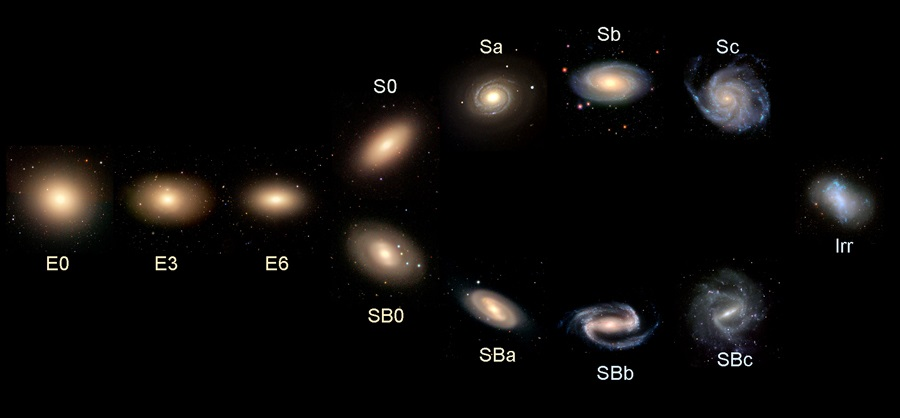
\includegraphics[width=0.8\textwidth]{Imagens/HubbleTuningFork.jpg} 
  \caption[Esquema de Hubble de classificação de galáxias.]{Representação esquemática de classificação das galáxias\footnotemark.} 
  \label{fig:esquema_hubble} 
\end{figure}
\footnotetext{Imagem feita pelo projeto Galaxy Zoo. Fonte: https://blog.galaxyzoo.org/tag/101.}

A análise da morfologia das galáxias é importante para o estudo de sua estrutura, informações sobre a cinemática, taxas de formação estelar e classificação de acordo com suas propriedades, identificando fases evolutivas e propriedades das estrelas. A categorização de galáxias é com base em suas formas, características físicas, ou também, pela atividade de buracos negros superdimensionados em suas regiões centrais.

\section{Classificação de galáxias}

Neste esquema, Figura~\ref{fig:esquema_hubble}, pioneiro de classificação morfológica proposto por Hubble, lembrando que não é evolutivo, há cinco grandes grupos: galáxias elípticas (E0 a E6), lenticulares (S0 e SB0), espirais barradas (SBa a SBc), espirais normais (Sa a Sc) e as irregulares (Irr). As galáxias elípticas possuem formato esférico ou elipsoidal, a propriedade de achatamento em seu formato tendendo do circular ao elíptico é dada por E\emph{n}, em que \emph{n} é a elipticidade projetada através da orientação dos planos de simetria (\emph{n} = 10(1 - b/a), b/a sendo a razão entre os eixos menor e maior da elipse), que determina sua classificação entre E0 a E6. Elas não possuem braços espirais, e ao longo de sua estrutura, há baixas concentrações de gás, poeira e estrelas jovens. As galáxias lenticulares possuem morfologia intermediária entre uma elíptica e espiral, possuindo formato de disco, porém com ausência de espiras.

\begin{figure}[h] 
  \centering 
  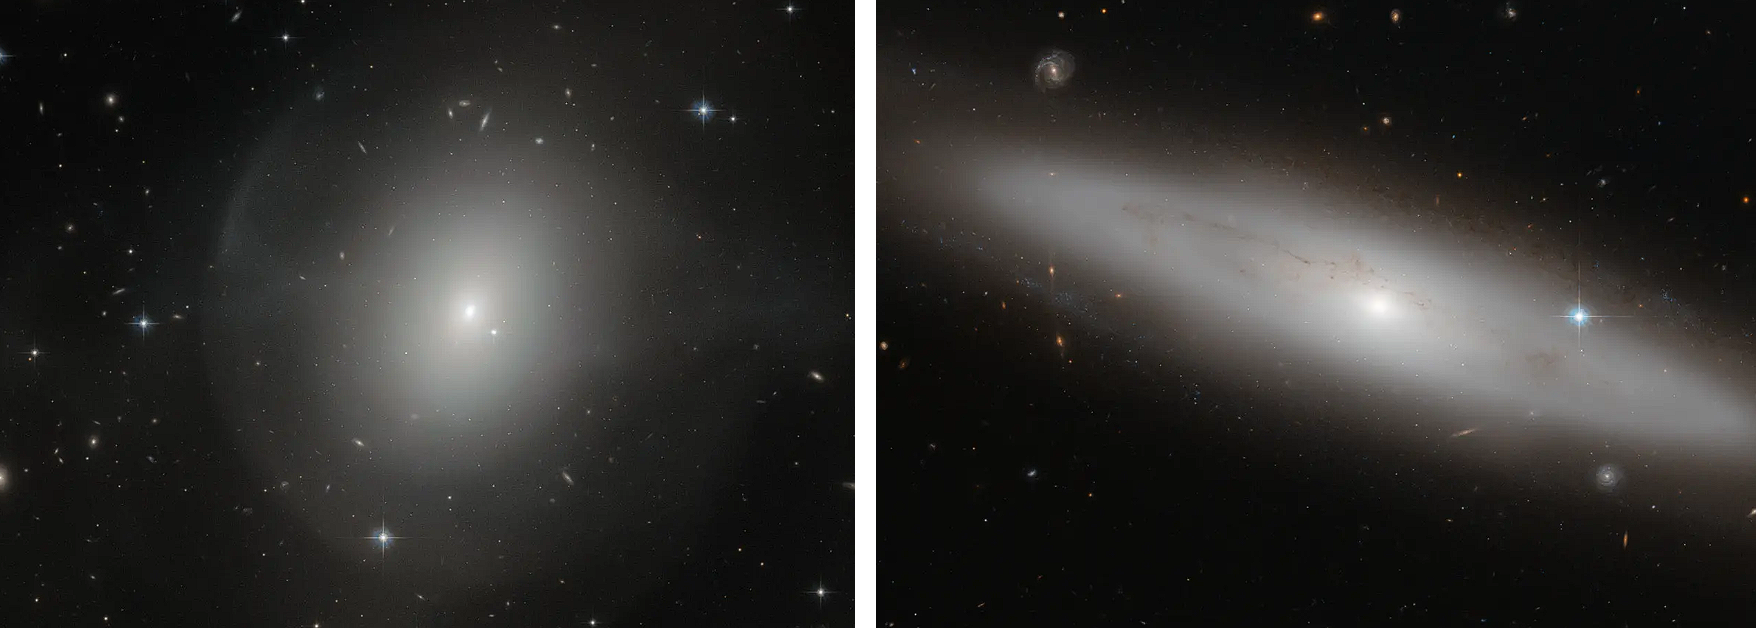
\includegraphics[width=0.8\textwidth]{Imagens/eliptica_lenticular.png} 
  \caption[Gálaxia elíptica NGC 2865 e gálaxia lenticular NGC 4886.]{A gálaxia elíptica NGC 2865, à esquerda, está localizada a 100 milhões de anos-luz de distância. A gálaxia lenticular NGC 4886, à direita, possui principalmente estrelas antigas, mas não braços espirais (imagens capturadas pelo Telescópio Espacial Hubble. Crédito: ESA/Hubble \& NASA).}
  \label{fig:eliptica_lenticular} 
\end{figure}

As galáxias espirais diferem entre si conforme o tamanho e formato do bojo (núcleo) e ao nível de desenvolvimento dos braços espirais. Estas galáxias apresentam um formato discoidal, possuem halo, braços espirais, disco, e bojo, onde há grande concentração de estrelas, podendo ser este barrado ou normal. Galáxias espirais barradas apresentam um núcleo estruturado em forma de barra e braços espirais, que comumente, partem das extremidades da barra. Galáxias espirais normais, possuem núcleo com formato comum e suas espiras partem tangencialmente desse núcleo em posições opostas. Ao analisar a idade das estrelas mais velhas em galáxias elípticas, observa-se que elas possuem, aproximadamente, a mesma idade das estrelas mais velhas das galáxias espirais, concluindo que ambos os tipos de galáxias tenham se originado na mesma época, quando a idade do universo era próxima de 1 bilhão de anos \cite{2023Muller}. O que determina a característica das estrelas de uma galáxia elíptica, predominantemente mais velhas, é que estas galáxias, em sua ``juventude'', tenham formado suas estrelas em um curto período de tempo, consumindo rapidamente grande parte de seu gás, enquanto que nas espirais, a taxa de formação estelar teria sido mais demorada, preservando parte de seu gás, e portanto, promovendo a criação de novas estrelas por mais tempo. Hubble chamou as galáxias elípticas de galáxias ``primitivas'' e as espirais de galáxias ``tardias''.

\begin{figure}[h] 
  \centering 
  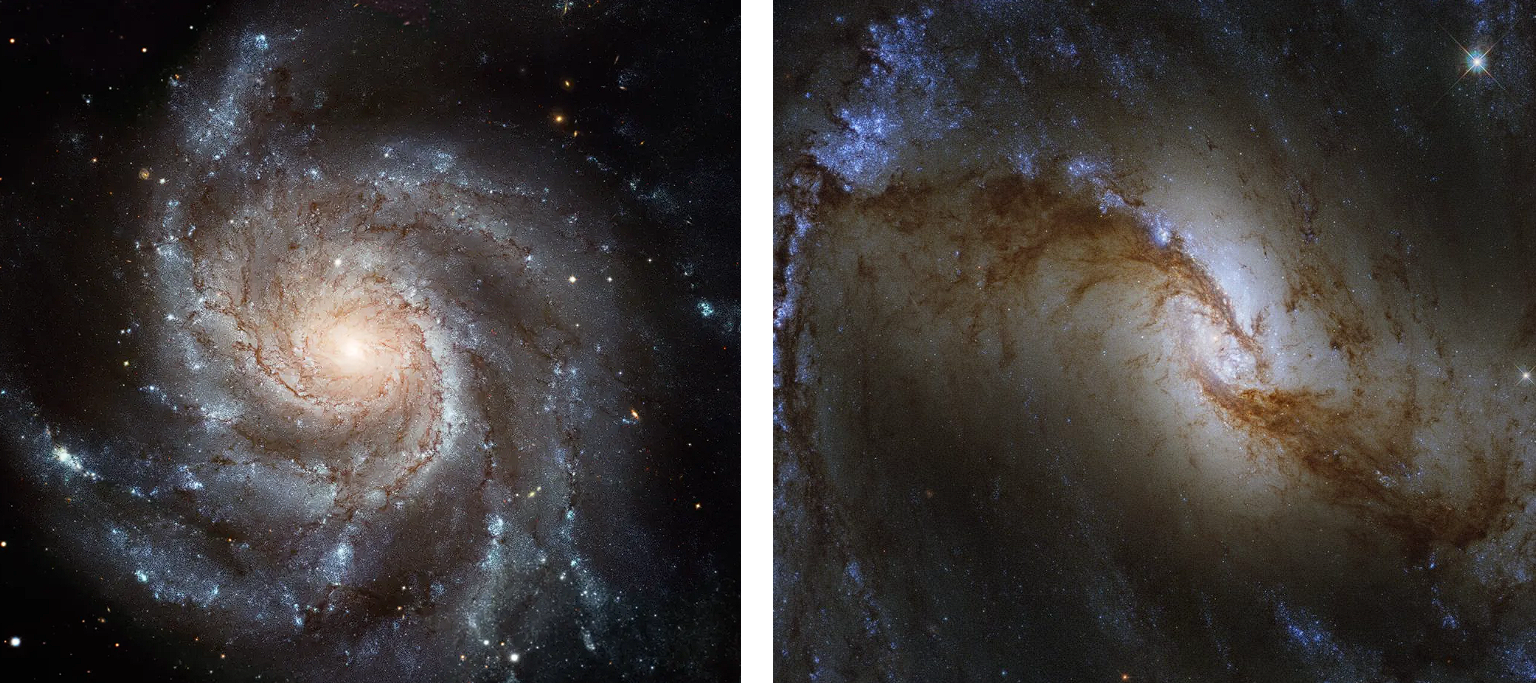
\includegraphics[width=0.8\textwidth]{Imagens/espirais.png} 
  \caption[Galáxia espiral M101 e espiral barrada NGC 1365.]{Galáxia espiral M101, à esquerda, conhecida como galáxia Pinwheel\footnotemark, está localizada a cerca de 27 milhões de anos-luz de distância na direção da constelação Ursa Maior (imagem capturada pelo Telescópio Espacial Hubble). A galáxia espiral barrada NGC 1365, à direita, localizada na constelação de Fornax, possui fortes colorações azuis, regiões onde estrelas acabaram de se formar (imagem capturada pelo Telescópio Espacial Hubble. Crédito: ESA/Hubble \& NASA).}
  \label{fig:espirais} 
\end{figure}
\footnotetext{Crédito: NASA, ESA, K. Kuntz (JHU), F. Bresolin (Universidade do Havaí), J. Laboratório de Propulsão a Jato (Trauger), J. Molde (NOAO), Y. H. Chu (Universidade de Illinois, Urbana) e STSci; Imagem CFHT: Telescópio Canadá-França-Havaí/J. C. Cuillandre/Coelum; NOAO Imagem: G. Jacoby, B. Bohannan, M. Hanna/NOAO/AURA/NSF.}

O quinto tipo morfológico de galáxias, inclusive bem diversificado, é foco deste trabalho: as irregulares (Irr). Como o próprio nome define, estas galáxias possuem uma estrutura peculiar, e geralmente, encontram-se junto a outras galáxias. As galáxias irregulares apresentam uma distribuição de luminosidade caótica, estrelas da população I e II (jovens e velhas), nuvens de gás ionizado distribuídas desarmoniosamente, geralmente intensa taxa de formação estelar, e são classificadas em dois tipos, Irregular I e Irregular II. O tipo Irr I, é o mais comum dos sistemas irregulares, possuem riqueza em gás e muitas estrelas jovens, enquanto que Irr II tem maior quantidade de poeira, são mais raras e vermelhas.

\begin{figure}[h] 
  \centering 
  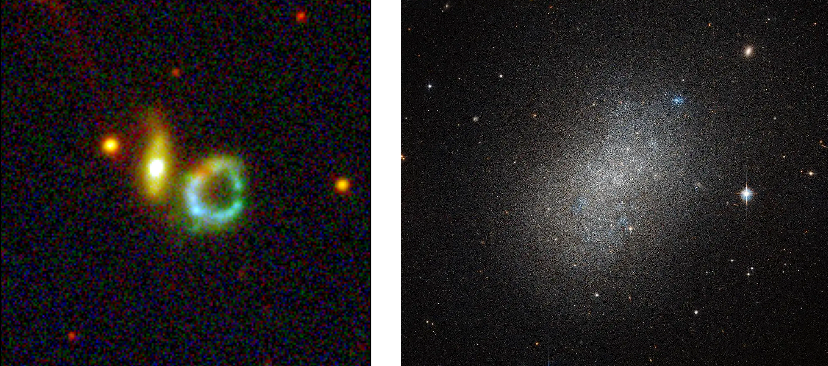
\includegraphics[width=0.8\textwidth]{Imagens/irregulares.png} 
  \caption[Gálaxia ARP 147 e gálaxia NGC 5264.]{A gálaxia irregular ARP 147, à esquerda, peculiar do tipo anelada (imagem capturada pelo telescópio T80S. Crédito: Southern Photometric Local Universe Survey). A gálaxia NGC 5264, à direita, irregular e anã (imagem capturada pelo Telescópio Espacial Hubble. Crédito: ESA/Hubble \& NASA).}
  \label{fig:irregulares} 
\end{figure}

\section{Interações entre galáxias}

Essas morfologias irregulares podem ser provocadas por perturbações, deformações e interações gravitacionais, como colisões (galáxia-galáxia), distorções das marés e canibalismo galáctico (fusão).

\begin{itemize}
	\item Colisões: As colisões entre galáxias são mais frequentes em aglomerados do que em regiões menos densas. Essas colisões potencialmente provocam mudanças na estrutura das galáxias interagentes, aumento de formação estelar e atividade nuclear, podendo ocorrer de forma lenta (\emph{v} orbital < \emph{v} interna) resultando em uma fusão, ou rápida  (\emph{v} orbital > \emph{v} interna) provocando perturbações morfológicas.
	\item Efeito de maré: Tende a deformar as galáxias que passam próximas entre si, puxando material galáctico, alongando-as, e a distribuição do material ao longo da interação é em parte, reflexo da conservação do \emph{momentum} angular das galaxias antes do choque.. Esse material, composto por poeira, gás, matéria escura e estrelas, dependendo, pode ser arrancado de uma galáxia (efeito \emph{tidal stripping}), se estendendo em formato de filamento, que se denomina caudas de maré. 
	\item Fusão: Refere-se à interação entre galáxias em que uma incorpora o material da interagente, destruindo sua estrutura. Resultados de simulações numéricas em computadores \cite{Barnes1996} mostram notavelmente a possibilidade de que colisões entre duas galáxias espirais, por exemplo, durante a interação, ocorre a retirada de gás, estrelas e poeira entre as galáxias, transformando-as em uma elíptica. Há estudos sobre as características peculiares em galáxias elípticas do tipo cD (gigantes) sugerindo que tenham se formado por canibalismo galáctico. Dependendo da fusão, se ocorrer um direcionamento de grande quantidade de material para a região central de uma elíptica resultante, há possibilidade de formação de um buraco negro.
\end{itemize}

\begin{figure}[h] 
  \centering 
  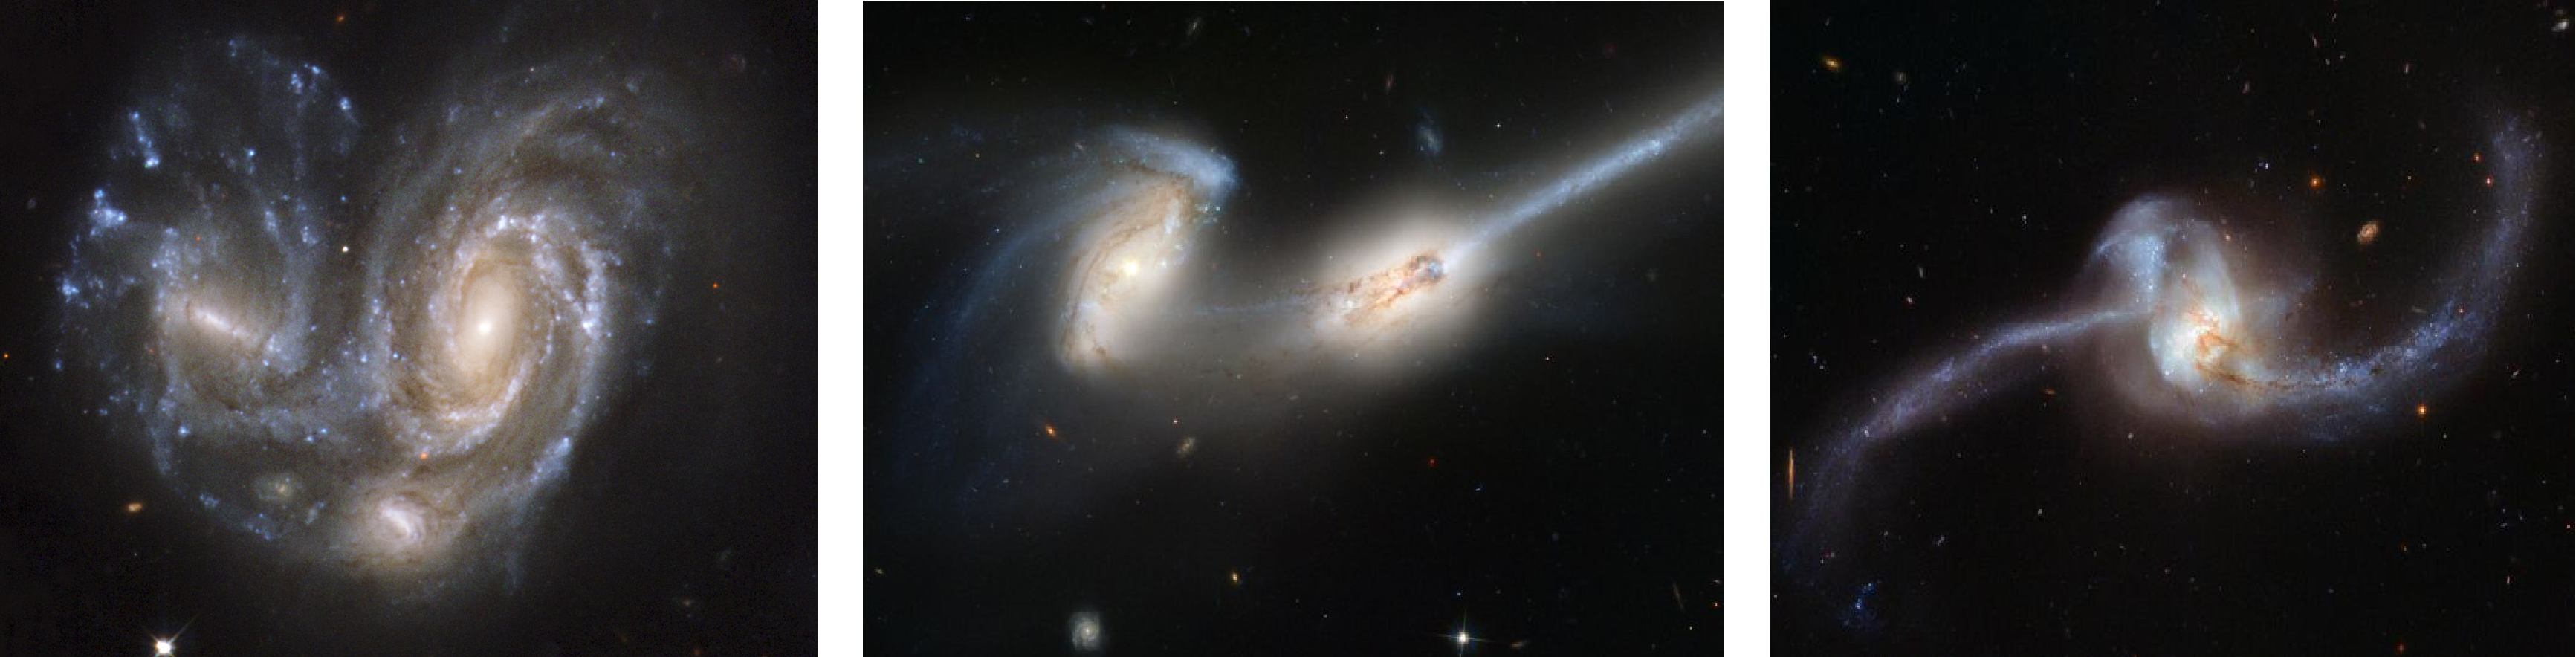
\includegraphics[width=1.0\textwidth]{Imagens/int_08.png} 
  \caption[Interação entre galáxias.]{Esquerda à direita: Colisão: NGC 6050 e IC 1179 são duas galáxias espirais que pelo processo de colisão, estão ligadas pelos seus braços espirais (NASA, ESA, the Hubble Heritage (STScI/AURA) Hubble Collaboration, and K. Noll (STScI)); Efeito de maré: observa-se as caudas longas de maré criadas nas galáxias espirais NGC 4676A e NGC 4676B, pela diferença relativa entre as forças gravitacionais nas partes próximas e distantes de cada uma (ACS Science \& Engineering Team, NASA Hubble Space Telescope); Fusão (ou merger): NGC 2623 se encontra no estágio final da fusão, onde se observa grande taxa de formação estelar pelas cores das estrelas e também o efeito das caudas de maré estendidas (ESA/Hubble e NASA).}
  \label{fig:interações} 
\end{figure}

Admiravelmente, quanto mais peculiar a estrutura de uma galáxia, mais marcante podem ter sido seus fenômenos e eventos. Muitos estudos, como de fotometria, morfologia, cinemática, espectrometria, são importantes para compreender os processos físico-químicos envolvidos nas interações que esses objetos peculiares passaram, ou estão passando, a fim de ilustrar e traçar sua fase evolutiva, prevendo também possibilidades futuras de interações.

\section{Motivação e objetivos}

A pesquisa e os estudos experimentais são resultados de anos de observações, aplicações teóricas e simulações computacionais, que formam juntos o grande banco de dados do que é o nosso universo, assim sendo a grande motivação deste trabalho. Esta pesquisa pretende fornecer pontos importantes sobre a fotometria de galáxias irregulares, com ênfase na família das galáxias peculiares aneladas (galáxia em anel ou \emph{ring galaxy}). As galáxias peculiares aneladas são fruto de interações e colisões entre galáxias, e nos permite, através das observações de perturbações em sua estrutura, estudar a evolução temporal da formação estelar dentro e fora do anel \cite{Appleton96}. A fotometria é o estudo das propriedades de distribuição de luz nas galáxias, e nos permite estudar a evolução e riqueza química destes objetos.

Neste estudo, analisamos 117 galáxias peculiares aneladas no hemisfério sul do universo local, a partir da base de dados de catálogos e atlas, e encontradas no levantamento fotométrico do Southern Photometric Local Universe Survey (S-PLUS), projeto de colaboração internacional fundada pela Universidade de São Paulo, Observatório Nacional,
Universidade Federal de Sergipe, Universidad de La Serena e Universidade Federal de Santa Catarina. No capítulo 2 apresentamos estudos de propriedades das galáxias aneladas e contribuições ao longo dos anos, explorando sua estrutura, propriedades estelares e evolução. No capítulo 3, abordamos sobre fotometria e as aberturas elípticas do S-PLUS utilizadas e suas propriedades para análise de dados. As amostras e suas respectivas abordagens de classificação e separação, utilizados nesta pesquisa, foram descritos no capítulo 4. No capítulo 5 são apresentados os resultados iniciais da qualidade fotométrica de abertura elíptica para estas galáxias de morfologia irregular, e no capítulo 6, as conclusões e contribuições, abrindo novas perspectivas para pesquisas futuras.



